\section{Linear Interpolation}

Linear interpolation is estimating the value between two data points given an input, $x$. The output $y$ is given by solving for the point along a line between the two given data points in the data set. In figure \ref{fig:linear}, two data points are given $(x_0,y_0)$ and $(x_1,y_1)$. 


\begin{figure}[H]
\begin{center}
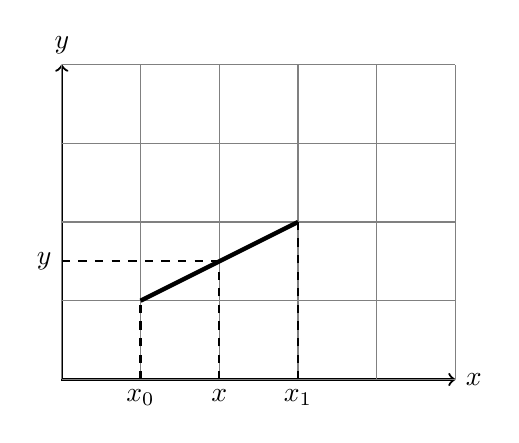
\begin{tikzpicture}
% Draw axes
\draw [<->,thick]
        (0,4) node (yaxis) [above] {$y$} |-
        (5,0) node (xaxis) [right] {$x$};
        
% Draw grid
\draw[gray, step=1cm] (0,0) grid (5,4);

\coordinate (x0) at (1,1);
\coordinate (x1) at (3,2);
\coordinate (xq) at (2,1.5);

% Draw path through points
        \draw [ultra thick]
        (x0) -- 
        %node[midway,above,sloped]
        %{\small $y=mx+b$}
        (x1);

% write x_0, x_1...
\draw[thick,dashed]
        (1,0) 
        node[below]{$x_0$} -- 
        (x0);
\draw[thick,dashed]
        (3,0) 
        node[below]{$x_1$} -- 
        (x1);
        
\draw[thick,dashed]
        (xq|-,0) 
        node[below]{$x$} -- 
        (xq);
\draw[thick,dashed]
        (0,1.5) 
        node[left]{$y$} -- 
        (xq);

% Draw points
\poi{1,1}
\poi{3,2}
\poi{2,1.5}

\end{tikzpicture}
\caption{Example dataset plot with splines}
\label{fig:linear}
\end{center}
\end{figure}

From the figure, similar triangles are used to relate the three points.

\begin{align}
	\frac{y-y_0}{x-x_0} 
	= \frac{y_1-y_0}{x_1-x_0}
\end{align}

Next, the output coordinate can be solved for:

\begin{align}
	y=y_0 + (x-x_0)\frac{y_1-y_0}{x_1-x_0}
\end{align}


\section{Quadratic Interpolation}